\documentclass{beamer}
\usepackage{graphicx}

\usetheme{Madrid}

\setbeamercolor{frametitle}{fg=blue}

\setbeamercolor{structure}{fg=yellow}

\title{Pokemon}
\author{tajemnica}
\date{\today}

\begin{document}

\begin{frame}
  \titlepage 
\end{frame}

\begin{frame}{Agenda}
  \tableofcontents 
\end{frame}


\begin{frame}{Cechy Pokemonow Wodnych}
  \begin{enumerate}
    \item \textbf{Srodowisko Wodne:} Pokemony Wodne zazwyczaj wystepuja w srodowiskach wodnych, takich jak jeziora, rzeki i oceany.

    \item \textbf{Ataki Wodne:} Czesto posiadaja potezne ataki wodne, takie jak Surf, Hydro Pump i Aqua Tail.

    \item \textbf{Adaptacyjnosc:} Sa znane ze swojej zdolnosci do adaptacji do roznych warunkow wodnych, co czyni je wszechstronnymi w roznych regionach.

    \item \textbf{Wrazliwosc na Typ Elektryczny:} Pomimo silnych atakow wodnych, sa podatne na ataki Typu Elektrycznego.

    \item \textbf{Roznorodnosc Gatunkow:} Typ Wodny obejmuje roznorodne gatunki Pokemonow, od małych ryb po gigantyczne stworzenia morskie.
  \end{enumerate}
\end{frame}


\section{Pokemony wodne}

\begin{frame}{Dratini - przyklad pokemona wodnego}
  \begin{figure}
    \centering
    
\includegraphics[width=0.7\textwidth]{dratini.jpg}
    \caption{dobra jest}
    \label{fig:dratini.jpg}
  \end{figure}
\end{frame}

\begin{frame}{Tabelka}
  \begin{table}
    \centering
    \begin{tabular}{|c|c|c|}
    \hline
    \textbf{Numer} & \textbf{Nazwa} & \textbf{Rodzaj} \\
    \hline
    007 & Squirtle & Water \\
    054 & Psyduck & Water \\
    060 & Poliwag & Water \\
    086 & Seel & Water \\
    090 & Shellder & Water \\
    116 & Horsea & Water \\
    118 & Goldeen & Water \\
    120 & Staryu & Water \\
    129 & Magikarp & Water \\
    147 & Dratini & Water \\
    \hline
  \end{tabular}
  \caption{Pokemony wodne}
    \label{tab:tabela0}
  \end{table}
\end{frame}


\begin{frame}{Cechy Pokemonow Lisciastych}
  \begin{enumerate}
    \item \textbf{Typ Roslinny:} Pokemon Lisciasty jest jednym z wielu typow pokemonow, charakteryzujacym sie zdolnosciami roslinnymi.

    \item \textbf{Ataki Roslinne:} Posiadaja ataki zwiazane z roslinnoscia, takie jak Vine Whip, Leaf Blade i Grass Knot.

    \item \textbf{Zdolnosci Lecznicze:} Niektore Pokemony Lisciaste maja zdolnosci lecznicze i moga pomagac w odbudowie zdrowia innych pokemonow.

    \item \textbf{Mimikryczne Umiejetnosci:} Potrafia przybierac ksztalt roslin lub kamuflowac sie wsrod zieleni, co pomaga im unikac przeciwnikow.

    \item \textbf{Ewolucje:} Pokemony Lisciaste maja rozne etapy ewolucji, co oznacza, ze moga rozwijac sie w bardziej zaawansowane formy.

    \item \textbf{Zastosowanie w Ekosystemie:} W swiecie Pokemon, niektore Pokemony Lisciaste pelnia role w ekosystemie, wplywajac na roslinnosc i przyrode.
  \end{enumerate}
\end{frame}


\section{Pokemony lisciaste}

\begin{frame}{Oddish - przyklad pokemona lisciastego}
  \begin{figure}
    \centering
    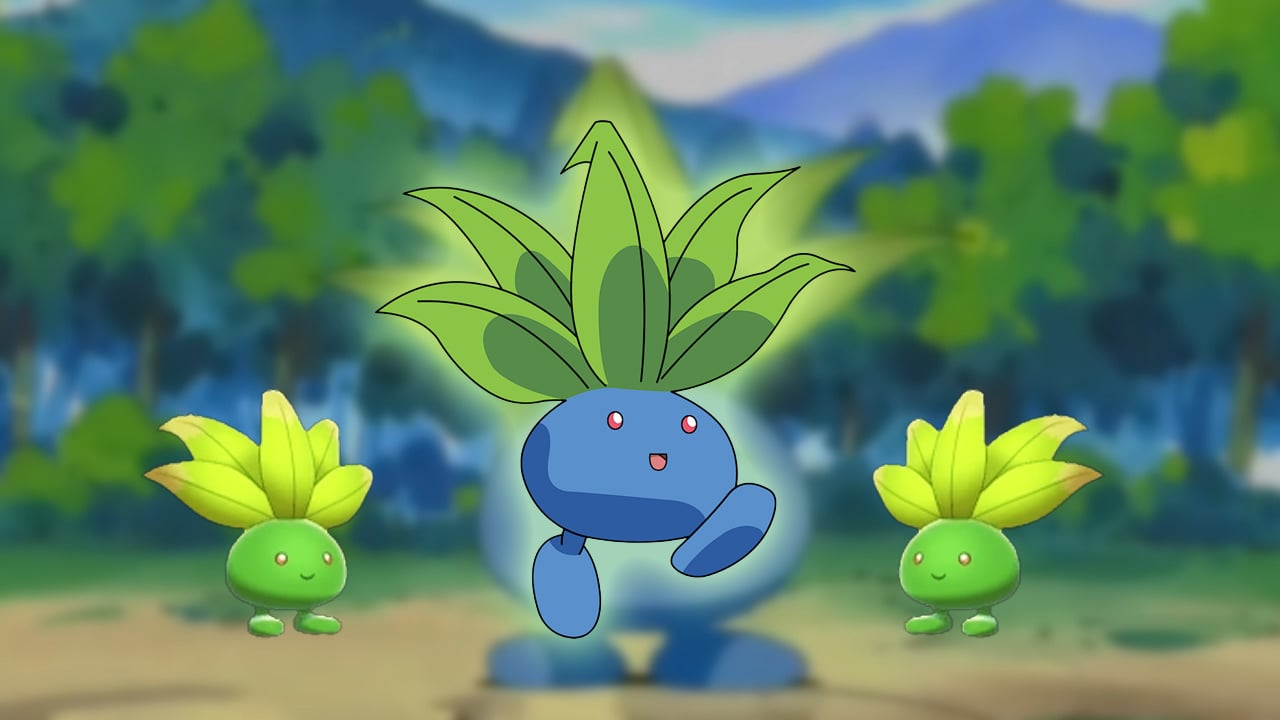
\includegraphics[width=0.7\textwidth]{oddish.jpg}
    \caption{mocny pokemon}
    \label{fig:oddish.jpg}
  \end{figure}
\end{frame}

\begin{frame}{Tabelka}
  \begin{table}
    \centering
    \begin{tabular}{|c|c|c|}
    \hline
    \textbf{Numer} & \textbf{Nazwa} & \textbf{Rodzaj} \\
    \hline
    001 & Bulbasaur & Grass/Poison \\
    002 & Ivysaur & Grass/Poison \\
    003 & Venusaur & Grass/Poison \\
    043 & Oddish & Grass/Poison \\
    044 & Gloom & Grass/Poison \\
    045 & Vileplume & Grass/Poison \\
    069 & Bellsprout & Grass/Poison \\
    070 & Weepinbell & Grass/Poison \\
    071 & Victreebel & Grass/Poison \\
    102 & Exeggcute & Grass/Psychic \\
    103 & Exeggutor & Grass/Psychic \\
    \hline
  \end{tabular}
  \caption{Pokemony lisciaste}
    \label{tab:tabela1}
  \end{table}
\end{frame}


\begin{frame}{Cechy Pokemonow Elektrycznych}
  \begin{enumerate}
    \item \textbf{Typ Elektryczny:} Pokemon Elektryczny jest jednym z wielu typow pokemonow, charakteryzujacym sie umiejetnosciami elektrycznymi.

    \item \textbf{Ataki Elektryczne:} Posiadaja silne ataki elektryczne, takie jak Thunderbolt, Thunder Shock i Electric Beam.

    \item \textbf{Szybkosc i Zwinnosc:} Wiele Pokemonow Elektrycznych jest znanych z szybkosci i zwinnosci, co pozwala im unikac atakow przeciwnikow.

    \item \textbf{Ewolucje:} Elektryczne Pokemony maja rozne etapy ewolucji, co oznacza, ze moga zmieniac sie w bardziej zaawansowane formy wraz z doswiadczeniem.

    \item \textbf{Wrazliwosc na Typ Ziemi:} Mimo swojej mocy, sa podatne na ataki Typu Ziemi.

    \item \textbf{Zastosowanie w Elektrycznych Strukturach:} Niektore Pokemon Elektryczne sa uzywane do zasilania elektrycznych struktur lub urzadzen w swiecie Pokemon.
  \end{enumerate}
\end{frame}


\section{Pokemony elektryczne}

\begin{frame}{Pikachu - przyklad pokemona elektrycznego}
  \begin{figure}
    \centering
    
\includegraphics[width=0.7\textwidth]{rys1.jpg}
    \caption{najpopularniejszy}
    \label{fig:rys1}
  \end{figure}
\end{frame}


\begin{frame}{Tabelka}
  \begin{table}
    \centering
    \begin{tabular}{|c|c|c|}
    \hline
    \textbf{Numer} & \textbf{Nazwa} & \textbf{Rodzaj} \\
    \hline
    025 & Pikachu & Electric \\
    026 & Raichu & Electric \\
    100 & Voltorb & Electric \\
    101 & Electrode & Electric \\
    125 & Electabuzz & Electric \\
    135 & Jolteon & Electric \\
    145 & Zapdos & Electric/Flying \\
    170 & Chinchou & Electric/Water \\
    172 & Pichu & Electric \\
    179 & Mareep & Electric \\
    \hline
  \end{tabular}
  \caption{Pokemony elektryczne}
    \label{tab:tabe}
  \end{table}
\end{frame}


\section{Podsumowanie}

\begin{frame}{Podsumowanie}
  \begin{itemize}
    \item :)
    \item Odniesienie do rysunku: Pikachu~\ref{fig:rys1}.
    \item Odniesienie do tabeli: Tabela pokemonow elektrycznych~\ref{tab:tabela1}.
  \end{itemize}
\end{frame}


\begin{frame}{Bibliografia i Przypisy}
  \begin{thebibliography}{99}
    \bibitem{Autor1} Autor1. \emph{Tytul 1.} Wydawnictwo, Rok.
    \bibitem{Autor2} Autor2. \emph{Tytul 2.} Wydawnictwo, Rok.
    \bibitem{Autor3} Autor3. \emph{Tytul 3.} Wydawnictwo, Rok.
    \bibitem{Autor4} Autor4. \emph{Tytul 4.} Wydawnictwo, Rok.
  \end{thebibliography}

\end{frame}
\end{document}
